\documentclass{article}

\usepackage[a4paper, left=1.5cm, right=1.5cm, top=1.0cm, bottom=1.0cm]{geometry}
\usepackage{graphicx} 
\usepackage{polski}
\usepackage[utf8]{inputenc}
\usepackage{setspace} % \onehalfspacing
\usepackage{lipsum}
\usepackage{array, xcolor}

\newcolumntype{C}[1]{>{\centering\arraybackslash}m{#1}}
\newcolumntype{R}[1]{>{\raggedleft\arraybackslash}m{#1}}

\onehalfspacing
\hyphenpenalty=5000
\tolerance=1000

\newcommand{\header}[1] 
{
	\textbf{\large #1}
	\vspace{0.005\textheight}
	\hrule 
	\vspace{0.005\textheight}
}

\pagenumbering{gobble} 
\begin{document}  
\noindent
\LARGE 
\centering
CURRICULUM VITAE \\
\large
\begin{tabular}{@{}p{0.70\textwidth} r}
	 \begin{minipage}{0.70\textwidth}
		\begin{tabular}{@{}l l} 
		\textbf{Imię i nazwisko}: 		& 	Bartłomiej Kordek\\
		\textbf{Data urodzenia}: & 1989.08.02\\
		\textbf{Adres}:		&	ul. Prosta 211, 05-152 Czosnów	\\
		\textbf{Telefon}:	& 507-832-154\\
		\textbf{E-mail}:	&	 bartekordek@gmail.com\\
		\end{tabular}	
	\end{minipage}
	
	& 
	\begin{minipage}{0.30\textwidth} 
		\begin{center}
			{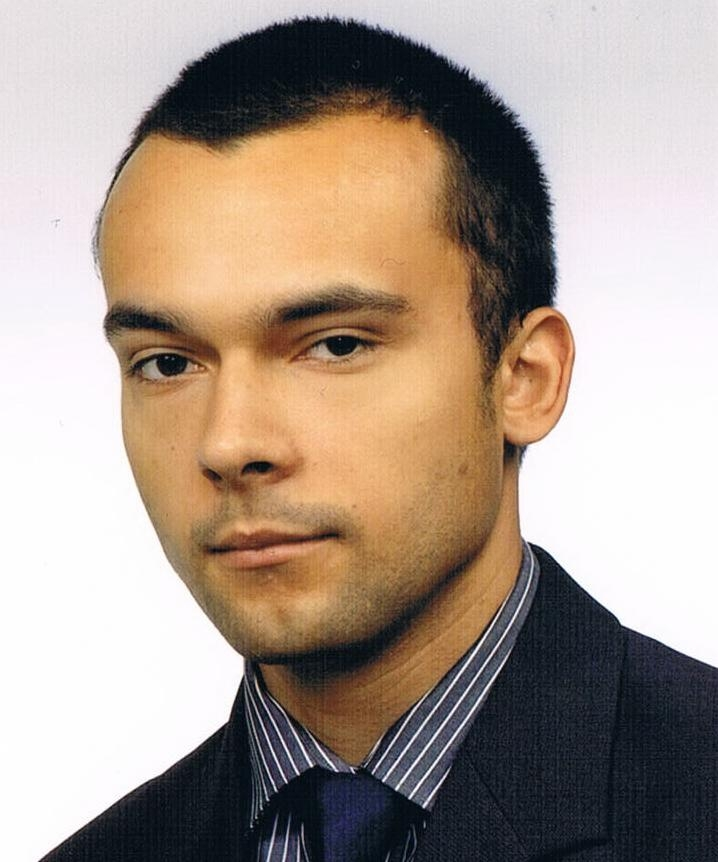
\includegraphics[width=0.70\textwidth]{./Picture}}
		\end{center} 
	\end{minipage}
\end{tabular}
\flushleft

\large
\header{Edukacja}
\begin{tabular}{@{} m{0.60\textwidth} R{0.37\textwidth} }
\textbf{Politechnika Warszawska}	& {2008 - 2012} \\
\end{tabular}
Inżynier Fizyki Technicznej, Specjalizacja: Materiały i Nanostruktury.\\
Tytuł pracy: "Eksperymentalna analiza korelacji między liniowym współczynnikiem rozszerzalności termicznej a temperaturą przejścia szklistego w wybranych amorficznych stopach metalicznych."
\begin{tabular}{@{} m{0.60\textwidth} R{0.37\textwidth} }
\textbf{Wyższa Szkoła Informatyki Stosowanej i Zarządzania}	& {2013 - dzisiaj} \\
\end{tabular}
Studia zaoczne - informatyka
\flushleft

\header{Doświadczenie}

\begin{tabular}{@{} m{0.60\textwidth} R{0.37\textwidth} }
\textbf{Samsung Electronics Polska}	& {2015-01 - 2015-03} 
\end{tabular}
Młodszy inżynier ds. produkcji oprogramowania\\
\begin{itemize}
	\item Zarządzanie i udoskonalanie środowiska testowego.
	\item Tworzenie oprogramowania w językach \texttt{C/C++}, Python i skrypty powłoki Bash.
	\item Zarządzanie i udoskonalanie serwera ciągłej integracji.
	\item Naprawianie błędów w oprogramowaniu.
	\item Przygotowywanie dokumentacji (\LaTeX).
\end{itemize}

\begin{tabular}{@{} m{0.60\textwidth} R{0.37\textwidth} }
	\textbf{Samsung Electronics Polska}	& {2014-08 - 2014-12} 
\end{tabular}
Praktykant\\
\begin{itemize}
	\item Zarządzanie i udoskonalanie serwera ciągłej integracji.
	\item Tworzenie oprogramowania ( skrypty \texttt{Bash}, \texttt{C\#}, \texttt{C/C++} i \texttt{Python}).
	\item Przygotowywanie dokumentacji (\LaTeX).
\end{itemize}

\begin{tabular}{@{} m{0.60\textwidth} R{0.37\textwidth} }
\textbf{Urząd Gminy} & {2013.03 - 2014-06} 
\end{tabular}
Pracownik biurowy\\
\begin{itemize}
	\item Tworzenie, edycja i zarządzanie dokumentami.
	\item Stworzenie i zarządzanie stroną internetową.
	\item Przyjmowanie interesantów.
	\item Konserwacja sprzętu elektronicznego.
\end{itemize}

\begin{tabular}{@{} m{0.60\textwidth} R{0.37\textwidth} }
\textbf{Instytut Technologii Elektrnonowej PAN} & {2011.07} 
\end{tabular}
Praktykant\\
\begin{itemize}
	\item Tworzenie oprogramowania nadzorującego serwomechanizmy używane w kalibracji i sterowania źródłem prądowym lasera (\texttt{Labview}).
	\item Utworzenie zwierciadła \emph{Bragga} dla wybranej długości światła widzialnego.
\end{itemize}

\textbf{\large Skills}
\vspace{0.005\textheight}
\hrule 

\begin{itemize}
	\item Pakiety Biurowe \texttt{Microsoft Office}, \texttt{Open Office}, \texttt{Libre Office}.
	\item Doświadczenie w tworzeniu dokumentów przy pomocy \LaTeX.
	\item Systemy operacyjne: \texttt{Linux} i \texttt{Windows}.
	\item Programowanie: \texttt{C}, \texttt{C++}, \texttt{C\#}, \texttt{Java}, skrypty (\texttt{Bash}), \texttt{Labview\texttt} i \texttt{Python}.
	\item Programowanie mikrokontrolerów \texttt{AVR}.
	\item Środowiska \texttt{ROOT} i \texttt{Mathematica}.
	\item Środowiska \texttt{Eclipse}, \texttt{VIM} and MS Visual Studio.
	\item Systemy kontroli wersji GIT i Perforce.
	\item Tworzenie stron (\texttt{HTML} and \texttt{CSS}).
	\item Podstawowa wiedza z zakresu elektroniki i elektrotechniki.
	\item Narzędzia \texttt{JIRA} and \texttt{FishEye}.
\end{itemize}

\header{Dodatkowe}
Prawo jazdy - kategoria B.
Znajomość język angielskiego - poziom B2.\\
Doświadczenie w użytkowaniu sprzętu laboratoryjnego: multimetry, oscyloskopy, źródła prądowe i generatory.
\header{Zainteresowania}
Muzyka, gitary, elektronika, programowanie, DIY, astronomia, fizyka, książki, filmy i sport.
\vspace{0.05\textheight}
\noindent\newline
\scriptsize
\begin{minipage}{\textwidth}
	 Wyrażam zgodę na przetwarzanie moich danych osobowych zawartych w mojej ofercie pracy dla potrzeb niezbędnych do realizacji procesu rekrutacji (zgodnie z Ustawą z dnia 29.08.1997 roku o Ochronie Danych Osobowych; tekst jednolity: Dz. U. z 2002r. Nr 101, poz. 926 ze zm.).
 \end{minipage}
 \end{document}

\end{minipage}

\end{document}
